\section{Dakkar}
\subsection{Descripci\'on de la problem\'atica}
La problem\'atica trata de una traves\'ia, la cual cuenta con \emph{n} cantidad de etapas. Para cada una de las etapas, se puede elegir recorrerla en alguno de los tres veh\'iculos disponibles: una BMX, una motocross o un buggy arenero. Cada uno de ellos permite concretar cada etapa en cantidades de tiempo diferentes.
Adem\'as, la cantidad de veces que se pueden usar la motocross y el buggy arenero est\'a acotada por \emph{k}$_m$ y \emph{k}$_b$ respectivamente.

Los \emph{tiempos} que le llevan a los veh\'iculos recorrer el trayecto var\'ian por cada etapa y son datos conocidos pasados por par\'ametro.

Se pide recorrer la traves\'ia, dentro de las restricciones, de modo que se utilice la menor cantidad de tiempo posible. Si existen dos (o m\'as) maneras de atravesarla dentro del tiempo
\'optimo, se pide devolver s\'olo una.

Se exige resolver la problem\'atica con una complejidad temporal de $O(n.k_m.k_b)$.\\

\bigskip

A continuaci\'on, se presenta un ejemplo sobre c\'omo resolver el problema, dado un caso espec\'ifico.\\

Dada una traves\'ia con 3 etapas (A, B y C), para las cuales se cuenta con 1 uso de la moto ($k_m$ = 1) y 2 usos del buggy ($k_b$ = 2), los tiempos que tarda cada veh\'iculo por cada etapa son los siguientes: \\

  \begin{figure}[h!]
   \begin{center}
 	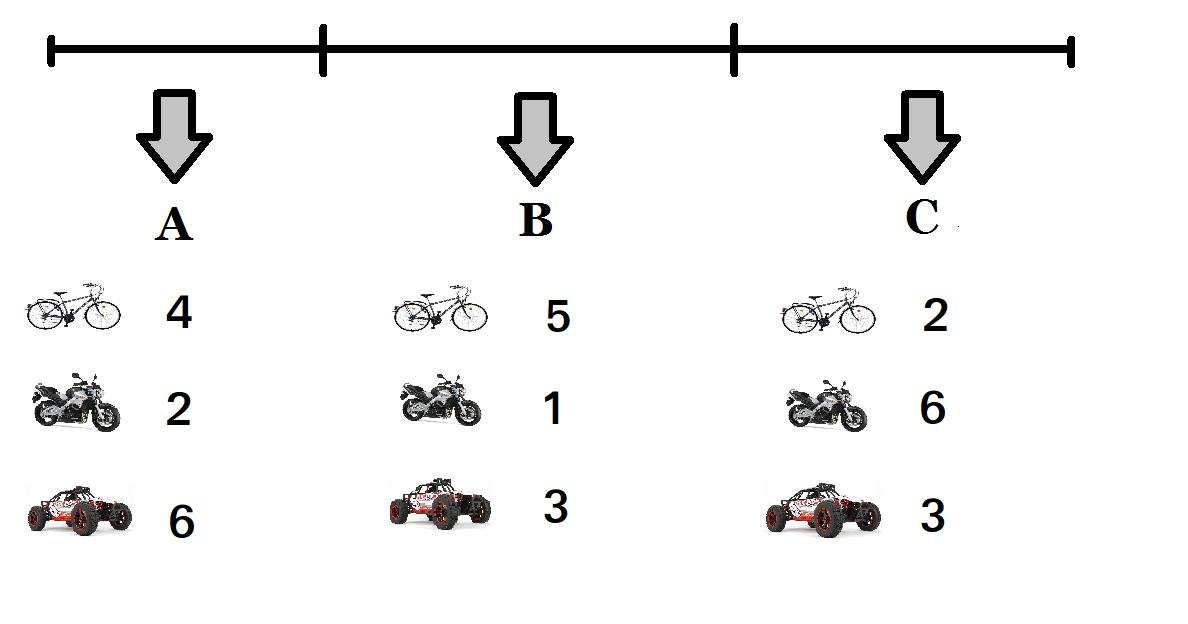
\includegraphics[scale=0.4]{imagenes/ej1/ejemplo.png}
% 	\caption{}
% 	\label{n.png}
   \end{center}
 \end{figure}



\newpage

En la siguiente tabla se muestran las diferentes elecciones que se pueden realizar,
teniendo en cuenta la cantidad de usos disponibles, indicando cu\'al es el tiempo total en cada caso.\\

\begin{table}[htb]
\centering
\begin{tabular}[c]{|l|l|l|l|l|}

		\hline
		Casos &\multicolumn{3}{|c|}{Veh\'iculo utilizado}& Tiempo total \\
		&\multicolumn{3}{|c|}{por etapa}&   \\
		\cline{2-4}
		&  $A$  &  $B$  &  $C$ &  \\
		\hline
		Caso 1& BMX & BMX & BMX & 11 \\
		\hline
		Caso 2& BMX & BMX & MOTO & 15 \\
		\hline
		Caso 3& BMX & BMX & BUGGY & 12 \\
		\hline
		\textbf{Caso 4}& \textbf{BMX} & \textbf{MOTO} & \textbf{BMX} & \textbf{7} \\
		\hline
		Caso 5& BMX & MOTO & BUGGY & 8 \\
		\hline		
		Caso 6& BMX & BUGGY & BMX & 9 \\
		\hline
		Caso 7& BMX & BUGGY & MOTO & 13 \\
		\hline
		Caso 8& BMX & BUGGY & BUGGY & 10 \\
		\hline
		Caso 9& MOTO & BMX & BMX & 9\\
		\hline
		Caso 10& MOTO & BMX & BUGGY & 10 \\
		\hline
		\textbf{Caso 11}& \textbf{MOTO} & \textbf{BUGGY} & \textbf{BMX} & \textbf{7} \\
		\hline
		Caso 12& MOTO & BUGGY & BUGGY & 8 \\
		\hline
		Caso 13& BUGGY & BMX & BMX & 13 \\
		\hline
		Caso 14& BUGGY & BMX & MOTO & 17 \\
		\hline
		Caso 15& BUGGY & BMX & BUGGY & 14 \\
		\hline
		Caso 16& BUGGY & MOTO & BMX & 9 \\
		\hline
		Caso 17& BUGGY & MOTO & BUGGY & 10 \\
		\hline
		Caso 18& BUGGY & BUGGY & BMX & 11 \\
		\hline
		Caso 19& BUGGY & BUGGY & MOTO & 15 \\
		\hline
		
	\end{tabular}
%\caption{Tabla muy sencilla.}
%\label{tabla:sencilla2}
\end{table}

En este ejemplo, la soluci\'on buscada, es decir, la \'optima, puede ser tanto el caso 4 como el 11, ya que ambos toman el mismo tiempo y respetan la cantidad de usos de buggy y moto posibles.
Por la formulaci\'on de nuestro algoritmo, nosotros devolvemos el caso 11.

\newpage
\subsection{Resoluci\'on propuesta y justificaci\'on}

Para resolver esta problem\'atica, optamos por implementar un algoritmo de \emph{Programaci\'on Din\'amica}.\\

Con el fin de encontrar el recorrido factible que emplee menos tiempo; debemos comparar, para cada etapa, cu\'al es el menor tiempo con el que puede recorrer el camino faltante eligiendo en la instancia actual uno de los tres veh\'iculos disponibles. Dado que la formulaci\'on de este problema es muy extensa, se realiz\'o una formulaci\'on recursiva de modo que para cada problema se le asigna un valor dependiendo de un subproblema menor. 

\subsubsection*{Formulaci\'on Recursiva}

Optamos por comenzar recorriendo desde la etapa n hasta la etapa 0; \emph{n} va a indicar la etapa actual, \emph{k$_m$} la cantidad de motos y \emph{k$_b$} la cantidad de buggys restantes que se pueden utilizar.

\begin{itemize}
\item[•]Cuando llegamos a la etapa \emph{n}$=0$ es porque terminamos todo el recorrido, de modo que el tiempo devuelto va a ser 0.

\item[•]Cuando \emph{k$_m$}$=0$ y \emph{k$_b$}$=0$ es porque la etapa actual (\emph{n}) y el recorrido restante (las \emph{n-1} etapas) lo vamos a tener que hacer s\'olo en bicicleta, sin importar el tiempo que conlleve ya que nos quedamos sin motos y buggys para usar.

\item[•]Cuando \emph{k$_m$}$=0$ y \emph{k$_b$}$\neq0$ es porque utilizamos la mayor cantidad de motos posibles y las \emph{n-1} etapas restantes -conjunto a la actual(\emph{n})- las vamos a tener que recorrer con Bicicleta o buggy. Por este motivo se elige la opci\'on con tiempo menor usando Bicicleta o buggy en la etapa \emph{n} y llamando recursivamente a la funci\'on para \emph{n-1} considerando esta elecci\'on.

\item[•]De modo an\'alogo, cuando \emph{k$_m$}$\neq0$ y \emph{k$_b$}$=0$ s\'olo vamos a contar con Motos y Bicicletas para la etapa actual y las \emph{n-1} etapas faltantes.

\item[•]En cambio, en caso contrario, todav\'ia tenemos disponible cantidad de los tres veh\'iculos. Por este motivo, se comparan los tres casos: empleando la Bicicleta en la etapa n, la Moto o el Buggy llamando recursivamente a la funci\'on para \emph{n-1} de modo que va a devolver el menor tiempo posible considerando la elecci\'on llevada a cabo.
\end{itemize}



\begin{equation*}
func(n, k_m, k_b) = 
\begin{cases} 
       0  & \mbox{si } n = 0  \\[2ex]
       tiempoBici(n) + f(n-1, 0, 0)  & \mbox{si } k_m=0 \wedge k_b=0 \\[2ex]
      min \left(
      \begin{split}
       tiempoBici(n) & + func(n-1, 0, k_b) , \\
       tiempobuggy(n) & + func(n-1, 0, k_b-1)
\end{split} \right) & \mbox{si } k_m=0 \wedge k_b\neq0 \\[3ex]
      min \left(
      \begin{split}
       tiempoBici(n) & + func(n-1, k_m, 0) , \\
       tiempoMoto(n) & + func(n-1, k_m-1, 0)
\end{split} \right) & \mbox{si } k_m\neq0 \wedge k_b=0 \\[3ex]
           min \left(
      \begin{split}
       tiempoBici(n) & + func(n-1, k_m, k_b) , \\
       tiempoMoto(n) & + func(n-1, k_m-1, k_b) , \\
       tiempobuggy(n) & + func(n-1, k_m, k_b-1)
\end{split} \right) & \mbox{sino}
\end{cases} 
\end{equation*}

Dado que los $n$, $k_m$ y $k_b$ iniciales van a ser los dados por par\'ametro y en el planteo de nuestra ecuaci\'on en la llamada recursiva n siempre decrementa en 1 y los dem\'as o bien quedan iguales o uno de ellos decrementa en uno, estos par\'ametros van a estar acotados por:

\begin{equation*}
\begin{array}{lllll}
0 & \leq & n &\leq & n_{_{parametro}} \\
0 & \leq & k_m & \leq & k_{m_{parametro}} \\
0 & \leq & k_b & \leq & k_{b_{parametro}}
\end{array}
\end{equation*}

\newpage

{\large\textbf{Teorema}}\\
La formulación recursiva planteada resuelve el problema.\\

{\large\textbf{Demostración}}\\
Para demostrar que el algoritmo resuelve, explotaremos la definición recursiva para aplicar inducción en la cantidad de etapas.\\
Entonces, queremos demostrar $P(n)=(\forall k_m, k_b) func(n, k_m, k_b)$ $obtiene$ $la$ $longitud$ $del$ $camino$ $minimo$.\\

\textbf{\emph{Caso base:}}\\
$P(0) = 0$\\
Vale, puesto que si no hay etapas, el camino mínimo tiene longitud 0, independientemente de la cantidad de buggys o motos de los que se disponga.\\

\textbf{\emph{Paso inductivo:}}\\
$P(n)\Rightarrow P(n+1)$\\
Primero vamos a mencionar que este problema cumple con el principio de optimalidad, es decir que, desde la etapa 0 hasta la i, la subsoluci\'on hallada, ser\'a \'optima.

Esto se puede ver en la tabla de anterior:

En el caso 4 y 11, si acotamos el problema a 2 etapas, ambas soluciones nos indican que el tiempo total ser\'ia 5, que es \'optimo.

Hasta la \emph{n-ésima} etapa, sabemos que contamos con el tiempo m\'inimo para cada decisi\'on posible en las n-1 etapas anteriores. Entonces por el principio de optimalidad, podemos agregar el tiempo m\'inimo de los posibles veh\'iculos, obteniendo una elecci\'on \'optima de \emph{n+1} etapas.

%Encontrándose en la \emph{n+1-ésima} etapa, el algoritmo calcula cuanto tiempo tomaría completar esa etapa (es decir, la \emph{longitud} entre la etapa anterior y la actual) para los distintos vehículos (tiempo que llamaremos $T_{v}$, donde $v$ es cada vehículo), y luego se invoca a s\'i mismo recursivamente, para cada posible decisión de que veh\'iculo utilizar. Finalmente, suma el tiempo $T_{v}$ al valor retornado a la función, para cada vehículo respectivo, y luego toma el mínimo de esos resultados.

%Sabemos que vale $P(n)$, es decir, que hasta \emph{n-ésima} etapa, el algoritmo ha tomado el camino mínimo para llegar a ella.

%Por el principio de optimalidad, si ya generó el camino mínimo hasta la \emph{n-ésima} etapa, solo debe ver qué vehiculo es conveniente usar entre la \emph{n+1-ésima} etapa y la \emph{n-ésima} etapa. Este es, efectivamente, su comportamiento.
Por lo tanto, vale $P(n) \Rightarrow P(n+1)$. $\square$\\

Resulta pertinenete destacar que el algoritmo resuelve de la misma manera que el \emph{Algoritmo de Bellman-Ford para caminos mínimos}, donde cada camino corresponde a las distintas decisiones posibles que se puedan tomar.

\subsubsection*{Diccionario a utilizar}

El diccionario que vamos a utilizar consiste en una matriz de $k_{m_{inicial}}$\texttt{x}$k_{b_{inicial}}$, en la que por cada posici\'on va a haber un contenedor de tama\~no $n_{_{inicial}}$ (lo cual forma un cubo) de modo que dentro de cada uno de ellos se va a poder almacenar el resultado de invocar a la funci\'on con estos tres par\'ametros.

\subsubsection*{Formulaci\'on Top Down}


Si analizamos el comportamiento de nuestra funci\'on recursiva como si fuera un algoritmo recursivo, podemos notar que la primer posici\'on del cubo que va a poder completar va a ser la de $(k_{m_{inicial}},k_{b_{inicial}},0)$, dado que para todas las guardas el primer caso que compara es usar la bicicleta. 

Luego, seguir\'a completando la matriz variando en orden ascendente el tercer par\'ametro y completando para todos los $k_m$ y $k_b$.

\subsubsection*{Formulaci\'on Bottom Up}

Una vez comprendido el comportamiento de la funci\'on, podemos establecer una manera de completar nuestro diccionario cubo de modo iterativo.\\

Primero completamos para $n=0$ todos los valores de $k_m$ y $k_b$. Notar que dados los \'indices que utilizamos a la hora de la implementaci\'on, cuando hablamos de $n=0$ nos referimos a la etapa 1 de la carrera (la \'ultima que vamos a recorrer), lo cual no es estrictamente el mismo resultado que el expuesto en la formulaci\'on recursiva. Sin embargo, podemos denotar esto como una diferencia que no afecta al funcionamiento del algoritmo.

Cuando $n=0$ simplemente vamos a asignar el veh\'iculo que presente menor tiempo para esta etapa, entre los disponibles bas\'andonos en los $k_m$ y $k_b$.

Luego para $n=1$, debemos considerar el costo m\'inimo entre usar cada uno de los veh\'iculos disponibles para esta etapa sumado a su correspondiente costo m\'inimo de la etapa anterior.

Continuamos con las iteraciones hasta llegar a $n=n_{_{parametro}}$.\\

Cuando contamos con la matriz Diccionario completa, nuestro resultado va a estar ubicado en la posici\'on $(k_{m_{parametro}},k_{b_{parametro}},n_{_{parametro}})$.\\

Al ingresar los datos dentro del diccionario de esta manera, lo \'unico que hacemos es invertir el orden de llenado. Es por este motivo que estamos cumpliendo con el mismo comportamiento de la funci\'on recursiva ya mencionada. Como ya pudimos asegurar que la formulaci\'on recursiva resolv\'ia de manera correcta la problem\'atica planteada, estamos en condiciones de afirmar que completar el diccionario en el orden inverso tambi\'en resuelve el ejercicio.\\

Con el fin de poder calcular el camino una vez obtenida la cantidad de tiempo menor para realizar el trayecto, en cada posici\'on del diccionario no s\'olo guardamos el tiempo empleado para llegar hasta ah\'i sino que tambi\'en cu\'al fue su situaci\'on inmediatamente anterior.\\

De este modo, recorremos la matriz  desde la posici\'on $(k_{m_{parametro}},k_{b_{parametro}},n_{_{parametro}})$ hacia la situaci\'on que indica la misma, y as\'i sucesivamente. De este modo obtenemos las elecciones hechas desde la \'ultima etapa hasta la primera.

\subsubsection*{PseudoC\'odigo}

\IncMargin{1em}
\begin{algorithm}
\SetKwData{Left}{left}\SetKwData{This}{this}\SetKwData{Up}{up}
\SetKwFunction{Union}{Union}\SetKwFunction{FindCompress}{FindCompress}
\SetKwInOut{Input}{input}\SetKwInOut{Output}{output}
\Input{int $n$, $k_m$, $k_b$ , lista$<$BMX, Moto, Buggy$>$ $datosPorEtapas$}
\BlankLine
\BlankLine
\For{$etapa\leftarrow 0$ \KwTo $n$}{
	\For{$cmoto\leftarrow 0$ \KwTo $k_m$}{
		\For{$cbuggy\leftarrow 0$ \KwTo $k_b$}{
			\emph{$dicc(cmoto, cbuggy, etapa) \leftarrow$Elijo el m\'inimo entre los veh\'iculos disponibles para esta etapa sumado a lo que tarde en la anterior considerando esta elecci\'on}\;
			\emph{$dicc(cmoto, cbuggy, etapa) \leftarrow$Elecci\'on tomada de veh\'iculo}\;
		}
	}
}
\BlankLine
\emph{Recorrer el diccionario desde la posici\'on final para armar el recorrido}\;
\caption{Dakkar}%\label{algo_ej3}
\end{algorithm}\DecMargin{1em}

\newpage

\subsection{An\'alisis de la complejidad}

\subsubsection{Complejidad Temporal}

Como par\'ametro vamos a recibir $n$, $k_m$, $k_b$ y los tiempos necesarios para atravesar con cada veh\'iculo las \emph{n} etapas. Los tiempos los vamos a tener almacenados en un vector de tuplas, donde cada componente va a ser BMX, Moto y buggy.\\

Mediante tres \texttt{for}s anidados (primero por la cantidad de etapas, despu\'es por la cantidad de motos y por \'ultimo la cantidad de buggys), vamos a recorrer posici\'on a posici\'on nuestra matriz de vectores (cubo). Comenzando en la posici\'on $(0,0,0)$ y finalizando en  $(k_{m},k_{b},n)$.

Dentro de cada iteraci\'on, lo que vamos a hacer es completar la posici\'on del diccionario correspondiente acorde indica el planteo recursivo, con la salvedad de que cada casillero representa cu\'anto nos cuesta llegar a la siguiente etapa, es decir, que la posici\'on $(k_{m},k_{b},n)$ tendr\'a lo que cueste ir de la etapa n a la etapa n+1, usando la cantidad de Motos y Buggys correspondiente.\\


En todas las iteraciones, escribiremos en el diccionario bajo la clave:  $(k{_m}, k{_b}, n)$. En cada posici\'on vamos a poner un par: la primera posici\'on corresponde al valor del tiempo y la segunda al indicador de la posici\'on inmediatamente anterior.\\

Para escribir la \emph{primer posici\'on} vamos a seguir las siguientes reglas:

\begin{itemize}
\item Si $n=0 \wedge k_m=0 \wedge k_b=0$ escribimos el tiempo que le lleva a la BMX para ir de $0$ a $1$
\item Si $n=0 \wedge k_m=0 \wedge k_b\neq0$ escribimos el tiempo que sea menor para ir  de $0$ a $1$ entre BMX y Buggy
\item Si $n=0 \wedge k_m\neq0 \wedge k_b=0$ escribimos el tiempo que sea menor para ir  de $0$ a $1$ entre BMX y Moto
\item Si $n=0 \wedge k_m\neq0 \wedge k_b\neq0$ escribimos el tiempo que sea menor para ir  de $0$ a $1$ entre BMX, Buggy y Moto
\item Si $n\neq0 \wedge k_m=0 \wedge k_b=0$ escribimos el tiempo que le lleva a la BMX para ir de $n$ a $n+1$ + $dicc(m, b, n-1)$
\item Si $n\neq0 \wedge k_m=0 \wedge k_b\neq0$ escribimos el tiempo que sea menor para ir  de $n$ a $n+1$ entre $tiempo(BMX) + dicc(m, b, n-1)$ y $tiempo(Buggy) + dicc(m, b-1, n-1)$
\item Si $n\neq0 \wedge k_m\neq0 \wedge k_b=0$ escribimos el tiempo que sea menor para ir  de $n$ a $n+1$ entre $tiempo(BMX) + dicc(m, b, n-1)$ y $tiempo(Moto) + dicc(m-1, b, n-1)$
\item Si $n\neq0 \wedge k_m\neq0 \wedge k_b\neq0$ escribimos el tiempo que sea menor para ir  de $n$ a $n+1$ entre $tiempo(BMX) + dicc(m, b, n-1)$, $tiempo(Buggy) + dicc(m, b-1, n-1)$ y $tiempo(Moto) + dicc(m-1, b, n-1)$
\end{itemize}

Debido a la forma de completar el diccionario, todas estas asignaciones son operaciones con un costo de $\mathbf{O(1)}$. 

Esto se debe a que acceder al vector con todos los costos por etapa, sumar y buscar el m\'inimo entre enteros ( \href{http://www.cplusplus.com/reference/algorithm/min/}{min()} \footnote{http://www.cplusplus.com/reference/algorithm/min/}) son operaciones de costo: $O(1)$. Adem\'as, al buscar en el diccionario siempre lo hacemos en posiciones ya definidas lo cual tambi\'en presenta un costo de $O(1)$ debido a que es una matriz de vectores.\\

\newpage

Para la \emph{segunda posici\'on}, que representa la escritura para devolver el camino, lo que realizamos es dejar asentado cu\'antos Buggys y cu\'antas Motos quedan disponibles despu\'es de esta iteraci\'on. 

El costo de estas operaciones tambi\'en pertenece a $\mathbf{O(1)}$. Las mismas son operaciones elementales (asignaci\'on y suma de enteros) y un llamado a  \href{http://www.cplusplus.com/reference/utility/make_pair/}{make\_pair()} \footnote{http://www.cplusplus.com/reference/utility/make_pair/} que toma tiempo constante.\\



Finalmente retornamos el valor de $dicc(k_{m_{parametro}},k_{b_{parametro}},n_{_{parametro}})$\\

La complejidad resulta entonces: por cada etapa, por cada posible uso de moto, por cada posible uso de buggy, realizar operaciones en tiempo constante. De esto deducimos que la complejidad es de $\mathbf{O(k_{m} * k_{b} * n)}$, como se ped\'ia en el enunciado.

\subsubsection{Complejidad Espacial}
Dado que la estructura utilizada es una matriz (\texttt{vector$<$vector$>$}) de $m_k$x$m_b$, donde en cada posici\'on contamos con un arreglo de $n$ posiciones y una tupla ($O(1)$); su complejidad espacial es de $\mathbf{O(k_m * k_b * n)}$.

\newpage
\subsection{C\'odigo fuente}
	\begin{codesnippet}
	\begin{verbatim}
    struct datosPorEtapas{
        unsigned int bmx;
        unsigned int moto;
        unsigned int buggy;
    };
	\end{verbatim}
	\end{codesnippet}

	\begin{codesnippet}
	\begin{verbatim}
    int main(int argc, char const *argv[]){
        unsigned int etapas, cmoto, cbuggy;
        cin >> etapas >> cmoto >> cbuggy;
        deque<datosPorEtapas> datos;
        for (int i = 0; i < etapas; ++i){
            unsigned int bmx, moto, buggy;
            datosPorEtapas actual;
            cin >> actual.bmx >> actual.moto >> actual.buggy;
            datos.push_back(actual);
        }
        Matriz cubo;
    //iniciliazamos el cubo
        for (int i = 0; i <= cmoto; ++i){
            Filas fila;
            for (int j = 0; j <= cbuggy; ++j){
                Etapas etapa;
                for (int k = 0; k < etapas; ++k){
                    etapa.push_back(make_pair(0, make_pair(0, 0)));
                }
                fila.push_back(etapa);
            }
            cubo.push_back(fila);
        }
    //cout pedido
        cout << dakkar(etapas, cmoto, cbuggy, datos, cubo);
    //para devolver del comienzo hasta el final
        deque<int> usados;
        pair<int, int> recorrido;
        int cantMoto = cmoto, cantBuggy = cbuggy;
        for (int cantE = etapas-1; cantE >= 0; --cantE) {
            recorrido = cubo[cantMoto][cantBuggy][cantE].second;
            if(cantMoto > recorrido.first){
                cantMoto--;
                usados.push_front(2);
            }
            else if(cantBuggy > recorrido.second){
                cantBuggy--;
                usados.push_front(3);
            }
            else{
                usados.push_front(1);
            }
        }
        for (int i = 0; i < etapas; ++i) {
            cout << " " << usados[i];
        }
        cout << endl;
        return 0;}
	\end{verbatim}
	\end{codesnippet}

	\begin{codesnippet}
	\begin{verbatim}
    unsigned int dakkar(unsigned int etapas, unsigned int cmoto, unsigned int cbuggy,
     deque<datosPorEtapas>& datos, Matriz& cubo){
        int bici, moto, buggy;
        for (int n = 0; n < etapas; ++n){
            for (int m = 0; m <= cmoto; ++m){
                for (int b = 0; b <= cbuggy; ++b){
                //guardamos un link hacia el lugar de donde salimos
                    pair<int, int> par;
                    par.first = m;
                    par.second = b;
                //llenamos espacios triviales y luego sabemos cuales estan calculados,
                // para ahorrar rehacer las cuentas
                    if (n==0){
                        if(m == 0){
                            if(b == 0){
                                bici = datos[n].bmx;
                                cubo[m][b][n] = make_pair(bici, par);
                            }
                            else{
                                bici = datos[n].bmx;
                                buggy = datos[n].buggy;
                            //si elegimos el buggy guardamos esa decision
                                if(bici > buggy)
                                    par.second--;
                                cubo[m][b][n] = make_pair(min(bici, buggy), par);
                            }
                        }
                        else{
                            if(b == 0){
                                bici = datos[n].bmx;
                                moto = datos[n].moto;
                            //si elegimos la moto guardamos esa decision
                                if(bici > moto)
                                    par.first--;
                                cubo[m][b][n] = make_pair(min(bici, moto), par);
                            }
                            else{
                                bici = datos[n].bmx;
                                moto = datos[n].moto;
                                buggy = datos[n].buggy;
                            //guardamos lo que elegimos
                                if(bici > buggy || bici > moto)
                                    if(buggy > moto)
                                        par.first--;
                                    else
                                        par.second--;
                                cubo[m][b][n] = make_pair(min(min(bici, moto), buggy), par);
                            }
                        }
                    }
	\end{verbatim}
	\end{codesnippet}

	\begin{codesnippet}
	\begin{verbatim}
                    else{
                        if(m == 0){
                            if(b == 0){
                                bici = cubo[m][b][n-1].first + datos[n].bmx;
                                cubo[m][b][n] = make_pair(bici, par);
                            }
                            else{
                                bici = cubo[m][b][n-1].first + datos[n].bmx;
                                buggy = cubo[m][b-1][n-1].first + datos[n].buggy;
                            //si elegimos el buggy guardamos esa decision
                                if(bici > buggy)
                                    par.second--;
                                cubo[m][b][n] = make_pair(min(bici, buggy), par);
                            }
                        }
                        else{
                            if(b == 0){
                                bici = cubo[m][b][n-1].first + datos[n].bmx;
                                moto = cubo[m-1][b][n-1].first + datos[n].moto;
                            //si elegimos la moto guardamos esa decision
                                if(bici > moto)
                                    par.first--;
                                cubo[m][b][n] = make_pair(min(bici, moto), par);
                            }
                            else{
                                bici = cubo[m][b][n-1].first + datos[n].bmx;
                                moto = cubo[m-1][b][n-1].first + datos[n].moto;
                                buggy = cubo[m][b-1][n-1].first + datos[n].buggy;
                            //guardamos lo que elegimos
                                if(bici > buggy || bici > moto)
                                    if(buggy > moto)
                                        par.first--;
                                    else
                                        par.second--;
                                cubo[m][b][n] = make_pair(min(min(bici, moto), buggy), par);
                            }
                        }
                    }
                }
            }
        }
        return cubo[cmoto][cbuggy][etapas-1].first;
    }
	\end{verbatim}
	\end{codesnippet}

\newpage
\subsection{Experimentaci\'on}

\subsubsection{Constrastaci\'on Emp\'irica de la complejidad}


Para realizar la experimentaci\'on, generamos una serie de tests en los cuales fuimos aumentando progresivamente la cantidad de etapas ($n$).
Los tiempos que le toma a cada veh\'iculo recorrer cada etapa fueron elegidos aleatoriamente, con n\'umeros entre 1 y 10000, ya que no influyen en la complejidad del algoritmo. 
Esto se debe a que las operaciones entre ellos son de comparaci\'on, es decir que tienen una complejidad de $O(1)$.\\

Luego, comenzamos mirando el caso m\'as sencillo (\emph{mejor caso}), que se da cuando tanto $k_m$ como $k_b$ son igual a 0. Es decir, en todos los casos debemos usar la BMX. 
  
  La complejidad te\'orica planteada es de $O(n * k_m * k_b)$, por lo que se intuye que en este caso deber\'ia ser $O(n)$.\\
  
  Los tiempos de ejecuci\'on para cada etapa $n$ fueron:
  
  \begin{table}[htb]
  \centering
  \begin{tabular}[c]{|l|l|}

		\hline
n & Tiempo en segundos\\
		\hline
50	&	0.0000428063\\
		\hline
100	&	0.0000990471\\
		\hline
150	&	0.0001270313\\
		\hline
200	&	0.0001718291\\
		\hline
250	&	0.0002251666\\
		\hline
300	&	0.0002632707\\
		\hline
350	&	0.0003082768\\
		\hline
400	&	0.0003563523\\
		\hline
450	&	0.0003971006\\
		\hline
500	&	0.0004461637\\
		\hline
550	&	0.0004880608\\
		\hline
600	&	0.0005325091\\
		\hline
650	&	0.0005865319\\
		\hline
700	&	0.0006258109\\
		\hline
750	&	0.0006709416\\
		\hline
800	&	0.0007168112\\
		\hline
850	&	0.0007580348\\
		\hline
900	&	0.000803331\\
		\hline
950	&	0.0008650634\\
		\hline
1000	&	0.0008941003\\
		\hline

	\end{tabular}
	%\caption{Tabla muy sencilla.}
	%\label{tabla:n.png}
	\end{table}

\newpage
	
  \begin{figure}[h!]
   \begin{center}
 	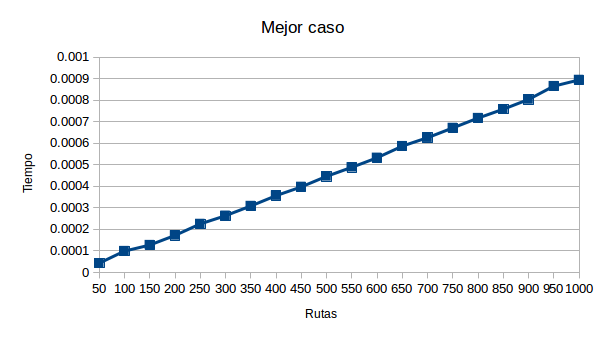
\includegraphics[scale=0.8]{imagenes/ej1/mejorCaso.png}
% 	\caption{}
% 	\label{n.png}
   \end{center}
 \end{figure}
 
  Como preve\'iamos, el gr\'afico tiene comportamiento lineal, lo cual es consistente con la cota te\'orica planteada.
  
  Luego, consideramos el \emph{peor caso} posible, que es el que iguala tanto $k_m$ como $k_b$ con $n$.
  Es decir, el caso en el que para cada etapa, tenemos la posiblidad de elegir cualquiera de las 3 opciones, BMX, motocross o buggy.\\
  
  Los tiempos de ejecuci\'on para cada etapa $n$ fueron:
  
  \begin{table}[htb]
  \centering
  \begin{tabular}[c]{|l|l|}

		\hline
n & Tiempo en segundos\\
		\hline
50	&	0.1744401\\
		\hline
100	&	1.733896\\
		\hline
150	&	6.082229\\
		\hline
200	&	14.68914\\
		\hline
250	&	29.19128\\
		\hline
300	&	50.62509\\
		\hline
350	&	81.18956\\
		\hline
400	&	121.5241\\
		\hline
450	&	173.8635\\
		\hline
500	&	239.492\\
		\hline
550	&	318.615\\
		\hline
600	&	420.213\\
		\hline
650	&	570.048\\
		\hline

	\end{tabular}
	%\caption{Tabla muy sencilla.}
	%\label{tabla:n.png}
	\end{table}
	
  \newpage

  \begin{figure}[h!]
   \begin{center}
	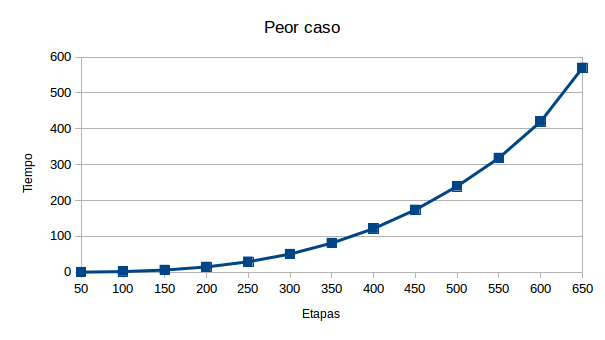
\includegraphics[scale=0.8]{imagenes/ej1/peorCaso1.png}
% 	\caption{}
% 	\label{n.png}
   \end{center}
  \end{figure}
  
  Como en este caso tanto $k_m$ como $k_b$ son iguales a $n$, la Cota de Complejidad planteada te\'oricamente ($O(n* k_m* k_b)$) es igual a $O(n^3)$.
  
  En el gr\'afico se aprecia una par\'abola creciente, pero no podemos asegurar que \'esta sea la que nosotros planteamos, ya que las curvas son similares a simple vista.

      
        Por lo explicado anteriormente, linealizamos los tiempos, dividiendo cada instancia por $n$.\\
        
  El gr\'afico resultante es el siguiente:
  
  \begin{figure}[h!]
   \begin{center}
	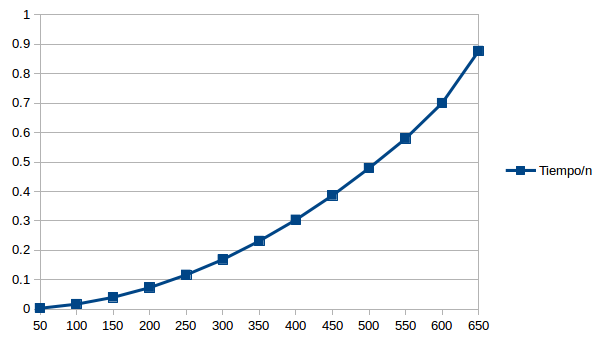
\includegraphics[scale=0.8]{imagenes/ej1/peorCaso2.png}
% 	\caption{}
% 	\label{n.png}
   \end{center}
  \end{figure}
  
      \newpage
  
  Este gr\'afico es similar al anterior, con una pendiende menos pronunciada.\\
  
  De todas formas, para asegurarnos que nuestra experimentaci\'on se condice con la Cota Te\'orica planteada, volvemos a dividir cada instancia por $n$ linealizando as\'i la muestra obtenida:\\
  
    \begin{figure}[h!]
   \begin{center}
	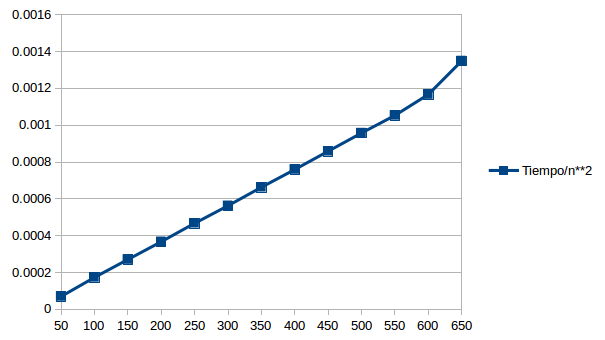
\includegraphics[scale=0.8]{imagenes/ej1/peorCaso3.png}
% 	\caption{}
% 	\label{n.png}
   \end{center}
  \end{figure}
  
  En efecto, este gr\'afico tiene comportamiento lineal, lo cual confirma nuestra afirmaci\'on y prueba emp\'iricamente nuestra cota de Complejidad Temporal Te\'orica.
    
  Luego, con el fin de comparar los tiempos de ejecuci\'on, se realiz\'o una \'ultima experimentaci\'on, en la cual se tomaron los mismos valores para $k_m$ y $k_b$, proporcionales al $n$ dado.\\  
  
  Como resultado se obtuvieron los siguientes valores:
    \begin{table}[htb]
  \centering
  \begin{tabular}[c]{|l|l|}

		\hline
n & Tiempo en segundos\\
		\hline
50	&	0.0015956707\\
		\hline
100	&	0.0152238567\\
		\hline
150	&	0.055239755\\
		\hline
200	&	0.132059613\\
		\hline
250	&	0.264843302\\
		\hline
300	&	0.464658156\\
		\hline
350	&	0.748833425\\
		\hline
400	&	1.13247454\\
		\hline
450	&	1.63054066\\
		\hline
500	&	2.28274084\\
		\hline
550	&	3.03236404\\
		\hline
600	&	3.84826384\\
		\hline
650	&	5.3375904\\
		\hline
700	&	6.2688524\\
		\hline
750	&	7.82798085\\
		\hline
800	&	9.62078432\\
		\hline
850	&	11.6278678182\\
		\hline
900	&	14.0280025641\\
		\hline
950	&	16.79448\\
		\hline
1000	&	19.80024\\
		\hline

	\end{tabular}
	%\caption{Tabla muy sencilla.}
	%\label{tabla:n.png}
	\end{table}
	
    \begin{figure}[h!]
   \begin{center}
	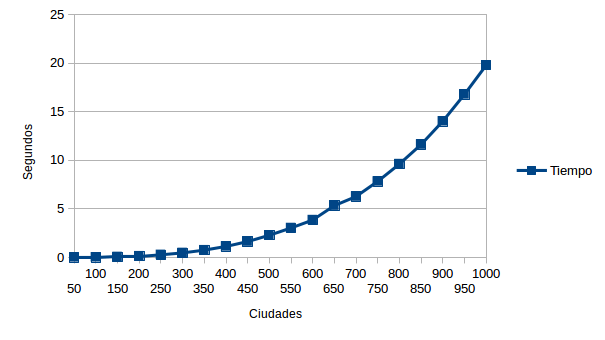
\includegraphics[scale=0.8]{imagenes/ej1/aleatorio1.png}
% 	\caption{}
% 	\label{n.png}
   \end{center}
  \end{figure}
    \newpage

  Como se ve, el gr\'afico tiene un comportamiento similar al del peor caso, pero los tiempos de ejecuci\'on son mucho menores, por lo que es evidente la influencia de $k_m$ y $k_b$ en la Cota Te\'orica planteada.
  